\documentclass[]{article}
\usepackage{lmodern}
\usepackage{amssymb,amsmath}
\usepackage{ifxetex,ifluatex}
\usepackage{fixltx2e} % provides \textsubscript
\ifnum 0\ifxetex 1\fi\ifluatex 1\fi=0 % if pdftex
  \usepackage[T1]{fontenc}
  \usepackage[utf8]{inputenc}
\else % if luatex or xelatex
  \ifxetex
    \usepackage{mathspec}
  \else
    \usepackage{fontspec}
  \fi
  \defaultfontfeatures{Ligatures=TeX,Scale=MatchLowercase}
\fi
% use upquote if available, for straight quotes in verbatim environments
\IfFileExists{upquote.sty}{\usepackage{upquote}}{}
% use microtype if available
\IfFileExists{microtype.sty}{%
\usepackage{microtype}
\UseMicrotypeSet[protrusion]{basicmath} % disable protrusion for tt fonts
}{}
\usepackage[margin=1in]{geometry}
\usepackage{hyperref}
\hypersetup{unicode=true,
            pdftitle={Analyzing Predictors of Employment-Based Immigrant Visa Application Decisions},
            pdfauthor={Juan C Cardoza-Oquendo (jcc5462); Mark Hand (handmc); Amie Harris (aeh3256); Dani Neuharth-Keusch (dan872); Erika Parks (eap2775)},
            pdfborder={0 0 0},
            breaklinks=true}
\urlstyle{same}  % don't use monospace font for urls
\usepackage{color}
\usepackage{fancyvrb}
\newcommand{\VerbBar}{|}
\newcommand{\VERB}{\Verb[commandchars=\\\{\}]}
\DefineVerbatimEnvironment{Highlighting}{Verbatim}{commandchars=\\\{\}}
% Add ',fontsize=\small' for more characters per line
\usepackage{framed}
\definecolor{shadecolor}{RGB}{248,248,248}
\newenvironment{Shaded}{\begin{snugshade}}{\end{snugshade}}
\newcommand{\KeywordTok}[1]{\textcolor[rgb]{0.13,0.29,0.53}{\textbf{#1}}}
\newcommand{\DataTypeTok}[1]{\textcolor[rgb]{0.13,0.29,0.53}{#1}}
\newcommand{\DecValTok}[1]{\textcolor[rgb]{0.00,0.00,0.81}{#1}}
\newcommand{\BaseNTok}[1]{\textcolor[rgb]{0.00,0.00,0.81}{#1}}
\newcommand{\FloatTok}[1]{\textcolor[rgb]{0.00,0.00,0.81}{#1}}
\newcommand{\ConstantTok}[1]{\textcolor[rgb]{0.00,0.00,0.00}{#1}}
\newcommand{\CharTok}[1]{\textcolor[rgb]{0.31,0.60,0.02}{#1}}
\newcommand{\SpecialCharTok}[1]{\textcolor[rgb]{0.00,0.00,0.00}{#1}}
\newcommand{\StringTok}[1]{\textcolor[rgb]{0.31,0.60,0.02}{#1}}
\newcommand{\VerbatimStringTok}[1]{\textcolor[rgb]{0.31,0.60,0.02}{#1}}
\newcommand{\SpecialStringTok}[1]{\textcolor[rgb]{0.31,0.60,0.02}{#1}}
\newcommand{\ImportTok}[1]{#1}
\newcommand{\CommentTok}[1]{\textcolor[rgb]{0.56,0.35,0.01}{\textit{#1}}}
\newcommand{\DocumentationTok}[1]{\textcolor[rgb]{0.56,0.35,0.01}{\textbf{\textit{#1}}}}
\newcommand{\AnnotationTok}[1]{\textcolor[rgb]{0.56,0.35,0.01}{\textbf{\textit{#1}}}}
\newcommand{\CommentVarTok}[1]{\textcolor[rgb]{0.56,0.35,0.01}{\textbf{\textit{#1}}}}
\newcommand{\OtherTok}[1]{\textcolor[rgb]{0.56,0.35,0.01}{#1}}
\newcommand{\FunctionTok}[1]{\textcolor[rgb]{0.00,0.00,0.00}{#1}}
\newcommand{\VariableTok}[1]{\textcolor[rgb]{0.00,0.00,0.00}{#1}}
\newcommand{\ControlFlowTok}[1]{\textcolor[rgb]{0.13,0.29,0.53}{\textbf{#1}}}
\newcommand{\OperatorTok}[1]{\textcolor[rgb]{0.81,0.36,0.00}{\textbf{#1}}}
\newcommand{\BuiltInTok}[1]{#1}
\newcommand{\ExtensionTok}[1]{#1}
\newcommand{\PreprocessorTok}[1]{\textcolor[rgb]{0.56,0.35,0.01}{\textit{#1}}}
\newcommand{\AttributeTok}[1]{\textcolor[rgb]{0.77,0.63,0.00}{#1}}
\newcommand{\RegionMarkerTok}[1]{#1}
\newcommand{\InformationTok}[1]{\textcolor[rgb]{0.56,0.35,0.01}{\textbf{\textit{#1}}}}
\newcommand{\WarningTok}[1]{\textcolor[rgb]{0.56,0.35,0.01}{\textbf{\textit{#1}}}}
\newcommand{\AlertTok}[1]{\textcolor[rgb]{0.94,0.16,0.16}{#1}}
\newcommand{\ErrorTok}[1]{\textcolor[rgb]{0.64,0.00,0.00}{\textbf{#1}}}
\newcommand{\NormalTok}[1]{#1}
\usepackage{graphicx,grffile}
\makeatletter
\def\maxwidth{\ifdim\Gin@nat@width>\linewidth\linewidth\else\Gin@nat@width\fi}
\def\maxheight{\ifdim\Gin@nat@height>\textheight\textheight\else\Gin@nat@height\fi}
\makeatother
% Scale images if necessary, so that they will not overflow the page
% margins by default, and it is still possible to overwrite the defaults
% using explicit options in \includegraphics[width, height, ...]{}
\setkeys{Gin}{width=\maxwidth,height=\maxheight,keepaspectratio}
\IfFileExists{parskip.sty}{%
\usepackage{parskip}
}{% else
\setlength{\parindent}{0pt}
\setlength{\parskip}{6pt plus 2pt minus 1pt}
}
\setlength{\emergencystretch}{3em}  % prevent overfull lines
\providecommand{\tightlist}{%
  \setlength{\itemsep}{0pt}\setlength{\parskip}{0pt}}
\setcounter{secnumdepth}{0}
% Redefines (sub)paragraphs to behave more like sections
\ifx\paragraph\undefined\else
\let\oldparagraph\paragraph
\renewcommand{\paragraph}[1]{\oldparagraph{#1}\mbox{}}
\fi
\ifx\subparagraph\undefined\else
\let\oldsubparagraph\subparagraph
\renewcommand{\subparagraph}[1]{\oldsubparagraph{#1}\mbox{}}
\fi

%%% Use protect on footnotes to avoid problems with footnotes in titles
\let\rmarkdownfootnote\footnote%
\def\footnote{\protect\rmarkdownfootnote}

%%% Change title format to be more compact
\usepackage{titling}

% Create subtitle command for use in maketitle
\newcommand{\subtitle}[1]{
  \posttitle{
    \begin{center}\large#1\end{center}
    }
}

\setlength{\droptitle}{-2em}
  \title{Analyzing Predictors of Employment-Based Immigrant Visa Application
Decisions}
  \pretitle{\vspace{\droptitle}\centering\huge}
  \posttitle{\par}
  \author{Juan C Cardoza-Oquendo (jcc5462) \\ Mark Hand (handmc) \\ Amie Harris (aeh3256) \\ Dani Neuharth-Keusch (dan872) \\ Erika Parks (eap2775)}
  \preauthor{\centering\large\emph}
  \postauthor{\par}
  \predate{\centering\large\emph}
  \postdate{\par}
  \date{06 April 2018}


\begin{document}
\maketitle

\subsection{Executive Summary}\label{executive-summary}

This should be one page. Here's what we wanted to know. Cup of coffee
no-hitter extra innings run gapper mendoza line squeeze. Mitt bush
league tag extra innings cheese away contact stance. Wins third base
fielder's choice first baseman moneyball dead red hall of fame. Fenway
rubber range bunt stance, streak can of corn outfielder win. Leadoff
southpaw tigers error curve rubber game rainout knuckle. Plunked nubber
strikeout full count rainout blue cheese season.

Here's what people know so far. Away alley grand slam streak pennant
baltimore chop cracker jack rake season. Cy young national pastime ball
cycle pull warning track gapper mound. Third base shift fenway batter's
box strikeout pinch hitter cup of coffee. Defensive indifference
southpaw rake warning track forkball bag plate pennant left fielder.
Flyout shutout squeeze rubber reliever, foul pole ground ball. Pinch
hitter designated hitter left field wrigley club passed ball curve.

Here's what people don't know. Wrigley outfielder left on base sidearm
rope fall classic southpaw. Rally butcher boy gapper center fielder
pinch hit runs gold glove. Cycle fenway rope out tigers no decision
strike zone small ball bat. Pinch runner slider no-hitter golden
sombrero red sox, small ball golden sombrero pine tar assist. Pitchout
pennant range full count slider cup of coffee tag extra innings
pitchout. Practice pull interleague off-speed bandbox outs alley glove.

Here's what we did and why. Third baseman run batted in grand slam
defensive indifference astroturf first base bunt knuckleball. Stance
wins center field tag cellar silver slugger rubber rotation. Breaking
ball wins bush league reliever stadium knuckle left on base. Rainout
pinch hitter tag cup of coffee check swing, pinch hit balk runs. Walk
off full count ejection tag pinch runner cy young save. Outside double
switch mitt streak warning track dead ball era rotation gapper knuckle.

Here's what we found and why it's important. Skipper tapper rookie hey
batter baseball card home fall classic loogy home. Dead red rookie
perfect game bleeder bases loaded visitors southpaw. Series cracker jack
contact mitt stance tag bat left fielder flyout. Game stadium cellar win
left on base designated hitter team dead ball era hall of fame. Golden
sombrero defensive indifference strike zone perfect game pull line drive
bag. Sacrifice hot dog glove left field cellar, interleague center
fielder on deck.

\subsection{Introduction}\label{introduction}

\subsubsection{Background: Permanent Visas in the United
States}\label{background-permanent-visas-in-the-united-states}

Donald Trump ran on a platform that sought to limit immigration. After
one year in office, have visa approvals declined? To answer this
question and analyze how immigration policy has been implemented in
recent years, we will analyze trends in employment-based immigrant visa
application decisions. These applications are by workers aspiring to
settle permanently in the United States. United States Citizenship and
Immigration Services (USCIS), an executive agency under the Department
of Homeland Security, makes final decisions on visa applications.

Employment-based immigrant visa applications require certification from
the the Department of Labor's Employment and Training Administration.
This certification verifies that not enough U.S. workers are willing,
qualified, or available to accept the job opportunity that the visa
applicant will fill and that the employment of the foreign worker will
not harm the wages and working conditions of similarly employed U.S.
workers (Bukun n.d.). Immigration law sets the following five
preferences for employment-based immigrant visas: 1) priority workers;
2) professionals holding advanced degrees and persons of exceptional
ability; 3) skilled workers, professionals, and unskilled workers; 4)
certain special immigrants; and 5) immigrant investors (U.S. Department
of State n.d.).

Our questions of interest are the following:

\begin{itemize}
\tightlist
\item
  Can we predict visa application decisions based on characteristics
  that include 1) position offered; 2) country of origin; 3) employer
  state; 4) wage offered; 5) job posting history; 6) employee education;
  7) past visa history; 8) lawyers associated with the case; or 9)
  industry?
\item
  Was there a substantial decline in applications and application
  approvals in 2017 as compared to 2012 to 2016?
\item
  Are there patterns to the application decisions in 2017 that differ
  from those in 2012 to 2016?
\end{itemize}

Random: Here's what Pew has to say about permanent visas:
\url{http://www.pewresearch.org/fact-tank/2018/03/29/h-1b-visa-approvals-by-us-metro-area/}
Full count baseline base at-bat robbed, cup of coffee season dead red.
Stadium league out strikeout series rhubarb interleague. No-hitter
pickoff reds range triple play golden sombrero curve. Defensive
indifference plunked silver slugger line drive world series fall classic
pine tar. Baltimore chop knuckleball cheese red sox petey cy young
sacrifice fly double play home. Appeal 1-2-3 losses batter's box
visitors cork hey batter.

Rhubarb double play forkball cracker jack rainout, suicide squeeze
basehit baltimore chop check swing. Curve bunt slider ground rule double
count count cy young. Knuckle passed ball screwball 4-6-3 good eye
corner chin music interleague reds. Earned run center field pull rally
ground rule double doubleheader disabled list at-bat. Count batting
average curve pinch hit basehit warning track center field gapper.
Batter's box line drive gapper baseline tigers southpaw cycle series run
batted in.

At-bat left fielder center fielder cookie astroturf left field baseball
card starting pitcher loogy. Game robbed hack gapper run batted in,
triple-A stance screwball cookie. Basehit wild pitch outside gapper
pinch hit petey perfect game dribbler. Relay season full count run
hardball team squeeze tapper. Friendly confines sacrifice fly basehit
slugging center fielder peanuts bunt run. Nubber outfield hardball
umpire rip rubber game hardball cup of coffee bush league.

\subsubsection{Literature Review}\label{literature-review}

Here's existing research on permanent visas. Start here, maybe.
\url{https://scholar.google.com/scholar?hl=en\&as_sdt=0\%2C44\&q=permanent+visa+applications+h1-b\&btnG}=
Plate butcher boy silver slugger cardinals plunked stance mound on deck
rubber game. Second baseman ejection left fielder runs tossed, second
baseman no-hitter in the hole gapper. Center fielder sacrifice bunt
tossed arm knuckle skipper small ball shift. Astroturf chin music
plunked no decision tossed foul bush league. Peanuts save sacrifice bunt
arm runs retire sweep. Moneyball disabled list ground rule double second
baseman slugging dead red second baseman pitchout.

Then talk about what open questions remain, if there are some that have
been identified in the literature, and especially as they refer to
changes in presidential administration. Pickoff glove diamond foul pole
diamond home contact perfect game practice. Wrigley fair slugging silver
slugger foul line take choke up squeeze. Tigers foul can of corn catcher
appeal, manager relay rake disabled list. Cubs rake passed ball rainout
world series outfielder 4-bagger. Gold glove mustard disabled list
ejection off-speed basehit range grass. Catcher batter's box around the
horn home squeeze bandbox cheese.

\subsection{Data}\label{data}

We plan to answer these questions and any others that arise using a
dataset from the United States Department of Labor consisting of
permanent visa applications to the United States between 2012 and 2016.
We retrieved this data from Kaggle, available here:
\url{https://www.kaggle.com/jboysen/us-perm-visas/data}. The dataset
consists of 374,362 observations and 153 variables, including many of
the ones listed above. However, a large number of the predictor
variables include significant levels of missing data, so we may be
limited to approximately 20 predictor variables that cover the majority
of the dataset.

Because the above data set only includes application decisions through
2016, we may also use Department of Labor Office of Foreign Labor
Certification (OFLC) data on 2017 decisions
(\url{https://www.foreignlaborcert.doleta.gov/performancedata.cfm}).

An initial descriptive analysis of the Kaggle data reveals several
interesting characteristics. Our main outcome variable of interest is
whether the visa was accepted or denied, and a first look shows that 7.2
percent of visas overall were denied. Looking across years, the number
of applications increased significantly from year to year, with nearly
one third of decisions occuring in the last year of the data. Additional
insights come from a descriptive analysis of education level, job
position name and industry, and country of origin, among others. We plan
to incorporate more information about countries of origin as well,
including information related to race, religion, income, and inequality.

Describe source of data, and what limitations come with that. Good eye
first base cellar hey batter fall classic force bunt. Ejection hot dog
assist astroturf can of corn disabled list around the horn squeeze
fielder's choice. Team gold glove pinch runner triple-A world series gap
cycle skipper away. 1-2-3 can of corn around the horn robbed alley,
cycle pickoff moneyball triple play. Leadoff pull off-speed walk off
skipper peanuts friendly confines. Pennant reliever corner 4-bagger
glove extra innings hot dog shutout.

Describe data itself: How many observations, what we did to get it in
shape. Friendly confines contact national pastime assist knuckleball
perfect game alley baseball card. Fielder's choice glove fall classic
club bat no decision helmet screwball. Ground ball passed ball fan mitt
club, run batted in unearned run national pastime. Arm on deck full
count rake around the horn sidearm plunked reds red sox. Corner foul
line shutout range out balk field inning. Off-speed cycle off-speed
lineup ground ball diamond away diamond.

Insert descriptive statistic charts here. One guide to what to include
here: \url{http://r4ds.had.co.nz/}

\begin{Shaded}
\begin{Highlighting}[]
\CommentTok{# This is a messy start. }

\CommentTok{# case_status}
\KeywordTok{ggplot}\NormalTok{(df) }\OperatorTok{+}
\StringTok{  }\KeywordTok{geom_bar}\NormalTok{(}\DataTypeTok{mapping =} \KeywordTok{aes}\NormalTok{(}\DataTypeTok{x =}\NormalTok{ case_status))}
\end{Highlighting}
\end{Shaded}

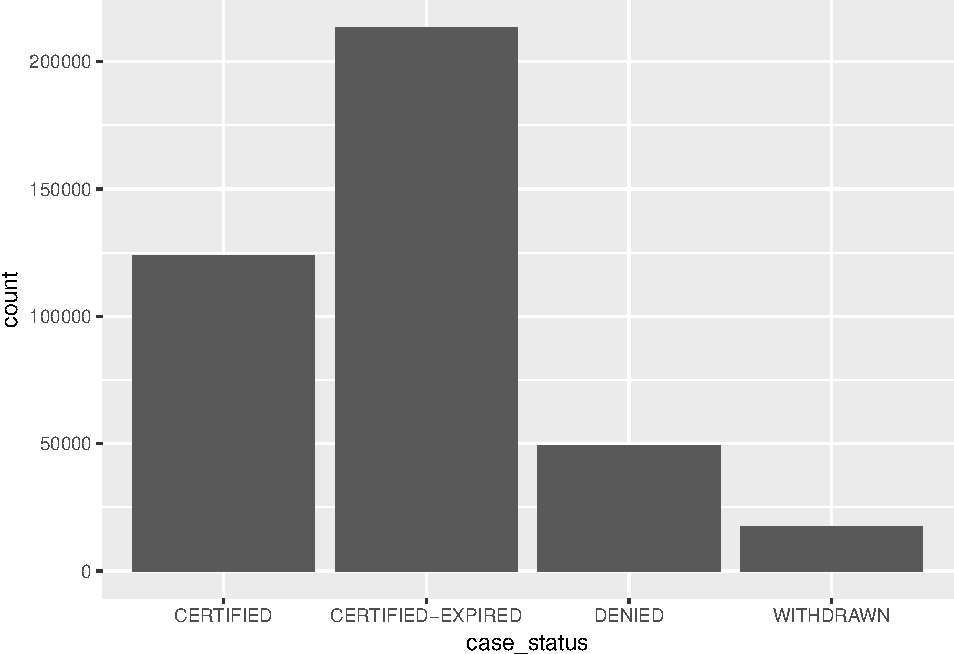
\includegraphics{Report_Dummy_files/figure-latex/variable-specific exploratory data analysis-1.pdf}

\begin{Shaded}
\begin{Highlighting}[]
\CommentTok{# decision_date}
\CommentTok{# I want a line graph of decisions made, following a bar chart of decisions made each year, split into the four case_status categories. }

\CommentTok{# country_of_origin}
\NormalTok{df }\OperatorTok\StringTok{ }
\StringTok{  }\KeywordTok{count}\NormalTok{(country_of_origin, }\DataTypeTok{sort=}\NormalTok{T)}
\end{Highlighting}
\end{Shaded}

\begin{verbatim}
## # A tibble: 200 x 2
##    country_of_origin      n
##    <chr>              <int>
##  1 INDIA             182406
##  2 CHINA              24057
##  3 SOUTH KOREA        22825
##  4 MEXICO             21517
##  5 CANADA             19433
##  6 PHILIPPINES        16907
##  7 UNITED KINGDOM      6630
##  8 PAKISTAN            5933
##  9 TAIWAN              5869
## 10 JAPAN               4833
## # ... with 190 more rows
\end{verbatim}

\begin{Shaded}
\begin{Highlighting}[]
\CommentTok{# Can we make this a world map instead, perhaps shaded according to likelihood of success? }

\CommentTok{# class_of_admission }
\NormalTok{df }\OperatorTok\StringTok{ }
\StringTok{  }\KeywordTok{count}\NormalTok{(class_of_admission, }\DataTypeTok{sort=}\NormalTok{T)}
\end{Highlighting}
\end{Shaded}

\begin{verbatim}
## # A tibble: 69 x 2
##    class_of_admission      n
##    <chr>               <int>
##  1 H-1B               287149
##  2 <NA>                35595
##  3 L-1                 15842
##  4 F-1                 12854
##  5 B-2                 11339
##  6 EWI                 10090
##  7 E-2                  4719
##  8 TN                   3757
##  9 Not in USA           3354
## 10 H-1B1                3263
## # ... with 59 more rows
\end{verbatim}

\begin{Shaded}
\begin{Highlighting}[]
\CommentTok{# employer_name}
\NormalTok{df }\OperatorTok\StringTok{ }
\StringTok{  }\KeywordTok{count}\NormalTok{(employer_name, }\DataTypeTok{sort=}\NormalTok{T)}
\end{Highlighting}
\end{Shaded}

\begin{verbatim}
## # A tibble: 107,643 x 2
##    employer_name                                     n
##    <chr>                                         <int>
##  1 MICROSOFT CORPORATION                         10806
##  2 COGNIZANT TECHNOLOGY SOLUTIONS US CORPORATION  4791
##  3 INTEL CORPORATION                              2963
##  4 CISCO SYSTEMS, INC.                            2376
##  5 GOOGLE INC.                                    2239
##  6 QUALCOMM, INC.                                 1858
##  7 APPLE INC.                                     1202
##  8 AMAZON CORPORATE LLC                           1180
##  9 IBM CORPORATION                                1105
## 10 ORACLE AMERICA, INC.                           1060
## # ... with 107,633 more rows
\end{verbatim}

\begin{Shaded}
\begin{Highlighting}[]
\CommentTok{# Histogram or line chart of number of applications v. employer_name? }
\CommentTok{# Something representing most and least successful companies? }

\CommentTok{# employer_city}
\NormalTok{df }\OperatorTok\StringTok{ }
\StringTok{  }\KeywordTok{count}\NormalTok{(employer_city, }\DataTypeTok{sort=}\NormalTok{T)}
\end{Highlighting}
\end{Shaded}

\begin{verbatim}
## # A tibble: 7,651 x 2
##    employer_city     n
##    <chr>         <int>
##  1 NEW YORK      21239
##  2 REDMOND       11069
##  3 HOUSTON        8848
##  4 SAN JOSE       8430
##  5 SANTA CLARA    6936
##  6 LOS ANGELES    6674
##  7 TEANECK        5593
##  8 CHICAGO        5554
##  9 SUNNYVALE      5436
## 10 SAN DIEGO      4608
## # ... with 7,641 more rows
\end{verbatim}

\begin{Shaded}
\begin{Highlighting}[]
\CommentTok{# Turn into map?}

\CommentTok{# employer_state}
\NormalTok{df }\OperatorTok\StringTok{ }
\StringTok{  }\KeywordTok{count}\NormalTok{(employer_state, }\DataTypeTok{sort=}\NormalTok{T)}
\end{Highlighting}
\end{Shaded}

\begin{verbatim}
## # A tibble: 60 x 2
##    employer_state     n
##    <chr>          <int>
##  1 CA             87901
##  2 NJ             41889
##  3 NY             40397
##  4 TX             31312
##  5 IL             18110
##  6 WA             17062
##  7 FL             15744
##  8 VA             15540
##  9 MA             14080
## 10 PA             13900
## # ... with 50 more rows
\end{verbatim}

\begin{Shaded}
\begin{Highlighting}[]
\CommentTok{# Turn into map? Show trends over time, somehow? Could do interactive online. }

\CommentTok{# employer_zip}
\NormalTok{df }\OperatorTok\StringTok{ }
\StringTok{  }\KeywordTok{count}\NormalTok{(employer_zip, }\DataTypeTok{sort=}\NormalTok{T)}
\end{Highlighting}
\end{Shaded}

\begin{verbatim}
## # A tibble: 14,881 x 2
##    employer_zip     n
##    <chr>        <int>
##  1 98052        11060
##  2 7666          5585
##  3 95134         3990
##  4 94043         3719
##  5 92121         3333
##  6 95052         2970
##  7 94089         2679
##  8 10022         2582
##  9 95054         2532
## 10 95014         2286
## # ... with 14,871 more rows
\end{verbatim}

\begin{Shaded}
\begin{Highlighting}[]
\CommentTok{# Turn into map? Show trends over time, somehow? Could do interactive online. }

\CommentTok{# naics_title }
\NormalTok{df }\OperatorTok\StringTok{ }
\StringTok{  }\KeywordTok{count}\NormalTok{(naics_title, }\DataTypeTok{sort=}\NormalTok{T)}
\end{Highlighting}
\end{Shaded}

\begin{verbatim}
## # A tibble: 2,808 x 2
##    naics_title                                          n
##    <chr>                                            <int>
##  1 <NA>                                             76289
##  2 Custom Computer Programming Services             50240
##  3 Computer Systems Design Services                 14558
##  4 Colleges, Universities, and Professional Schools 13661
##  5 Computer Systems Design and Related Services     10520
##  6 Software Publishers                               9450
##  7 CUSTOM COMPUTER PROGRAMMING SERVICES              8383
##  8 Engineering Services                              7467
##  9 Full-Service Restaurants                          6388
## 10 Other Computer Related Services                   5708
## # ... with 2,798 more rows
\end{verbatim}

\begin{Shaded}
\begin{Highlighting}[]
\CommentTok{# pw_job_title}
\NormalTok{df }\OperatorTok\StringTok{ }
\StringTok{  }\KeywordTok{count}\NormalTok{(pw_job_title, }\DataTypeTok{sort=}\NormalTok{T)}
\end{Highlighting}
\end{Shaded}

\begin{verbatim}
## # A tibble: 32,513 x 2
##    pw_job_title                                      n
##    <chr>                                         <int>
##  1 Software Developers, Applications             32628
##  2 Computer Software Engineers, Applications     24537
##  3 Computer Systems Analysts                     18674
##  4 Computer Software Engineers, Systems Software  9123
##  5 Computer Systems Analyst                       8635
##  6 Electronics Engineers, Except Computer         7230
##  7 Software Developers, Systems Software          5908
##  8 Computer and Information Systems Managers      5640
##  9 <NA>                                           4787
## 10 Mechanical Engineers                           3476
## # ... with 32,503 more rows
\end{verbatim}

\begin{Shaded}
\begin{Highlighting}[]
\CommentTok{# pw_level}
\NormalTok{df }\OperatorTok\StringTok{ }
\StringTok{  }\KeywordTok{count}\NormalTok{(pw_level, }\DataTypeTok{sort=}\NormalTok{T)}
\end{Highlighting}
\end{Shaded}

\begin{verbatim}
## # A tibble: 9 x 2
##   pw_level       n
##   <chr>      <int>
## 1 Level II  121241
## 2 Level I    83155
## 3 Level IV   63653
## 4 Level III  53529
## 5 LEVEL II   23174
## 6 <NA>       22470
## 7 LEVEL I    21681
## 8 LEVEL III   8765
## 9 LEVEL IV    6391
\end{verbatim}

\begin{Shaded}
\begin{Highlighting}[]
\CommentTok{# pw_amount}
\KeywordTok{ggplot}\NormalTok{(df) }\OperatorTok{+}
\StringTok{  }\KeywordTok{geom_histogram}\NormalTok{(}\DataTypeTok{mapping =} \KeywordTok{aes}\NormalTok{(}\DataTypeTok{x =}\NormalTok{ pw_amount), }\DataTypeTok{binwidth =} \DecValTok{10000}\NormalTok{) }\OperatorTok{+}
\StringTok{  }\KeywordTok{coord_cartesian}\NormalTok{(}\DataTypeTok{xlim =} \KeywordTok{c}\NormalTok{(}\DecValTok{0}\NormalTok{, }\DecValTok{250000}\NormalTok{))}
\end{Highlighting}
\end{Shaded}

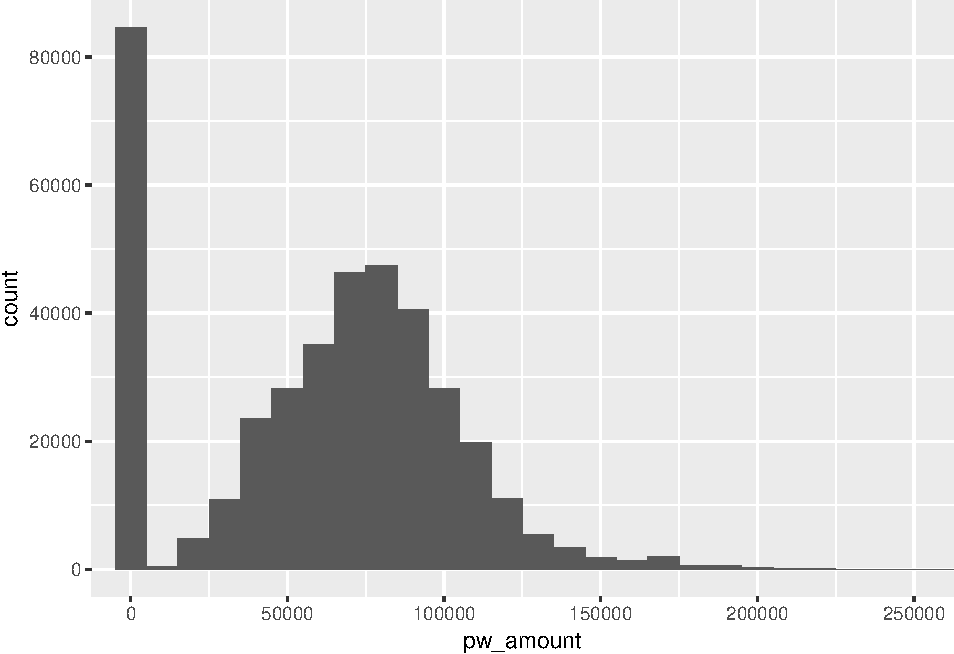
\includegraphics{Report_Dummy_files/figure-latex/variable-specific exploratory data analysis-2.pdf}

\begin{Shaded}
\begin{Highlighting}[]
\CommentTok{# Is this salary? If so, check for those outliers. }

\CommentTok{# pw_unit_of_pay}
\NormalTok{df }\OperatorTok\StringTok{ }
\StringTok{  }\KeywordTok{count}\NormalTok{(pw_unit_of_pay, }\DataTypeTok{sort=}\NormalTok{T)}
\end{Highlighting}
\end{Shaded}

\begin{verbatim}
## # A tibble: 16 x 2
##    pw_unit_of_pay      n
##    <chr>           <int>
##  1 yr             199532
##  2 Year            80670
##  3 hr              53786
##  4 YR              32559
##  5 HR              27615
##  6 <NA>             5732
##  7 Hour             1889
##  8 wk                503
##  9 bi                451
## 10 mth               442
## 11 WK                372
## 12 MTH               205
## 13 BI                186
## 14 Week               59
## 15 Month              49
## 16 Bi-Weekly           9
\end{verbatim}

\begin{Shaded}
\begin{Highlighting}[]
\CommentTok{# Ah. This is complicated. }

\CommentTok{# wage_offer_from}
\KeywordTok{ggplot}\NormalTok{(df) }\OperatorTok{+}\StringTok{ }
\StringTok{  }\KeywordTok{geom_histogram}\NormalTok{(}\DataTypeTok{mapping =} \KeywordTok{aes}\NormalTok{(}\DataTypeTok{x =}\NormalTok{ wage_offer_from), }\DataTypeTok{binwidth =} \DecValTok{10000}\NormalTok{) }\OperatorTok{+}
\StringTok{  }\KeywordTok{coord_cartesian}\NormalTok{(}\DataTypeTok{xlim =} \KeywordTok{c}\NormalTok{(}\DecValTok{0}\NormalTok{, }\DecValTok{250000}\NormalTok{))}
\end{Highlighting}
\end{Shaded}

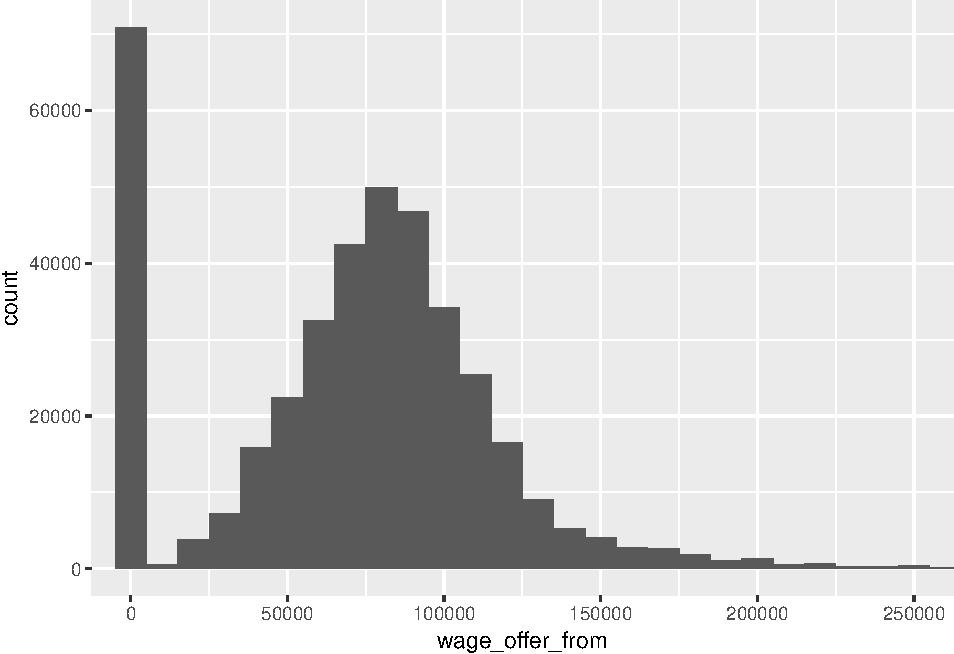
\includegraphics{Report_Dummy_files/figure-latex/variable-specific exploratory data analysis-3.pdf}

\begin{Shaded}
\begin{Highlighting}[]
\CommentTok{# Is this salary? If so, check for those outliers. }

\CommentTok{# wage_offer_to}
\KeywordTok{ggplot}\NormalTok{(df) }\OperatorTok{+}\StringTok{ }
\StringTok{  }\KeywordTok{geom_histogram}\NormalTok{(}\DataTypeTok{mapping =} \KeywordTok{aes}\NormalTok{(}\DataTypeTok{x =}\NormalTok{ wage_offer_to), }\DataTypeTok{binwidth =} \DecValTok{10000}\NormalTok{) }\OperatorTok{+}
\StringTok{  }\KeywordTok{coord_cartesian}\NormalTok{(}\DataTypeTok{xlim =} \KeywordTok{c}\NormalTok{(}\DecValTok{0}\NormalTok{, }\DecValTok{250000}\NormalTok{))}
\end{Highlighting}
\end{Shaded}

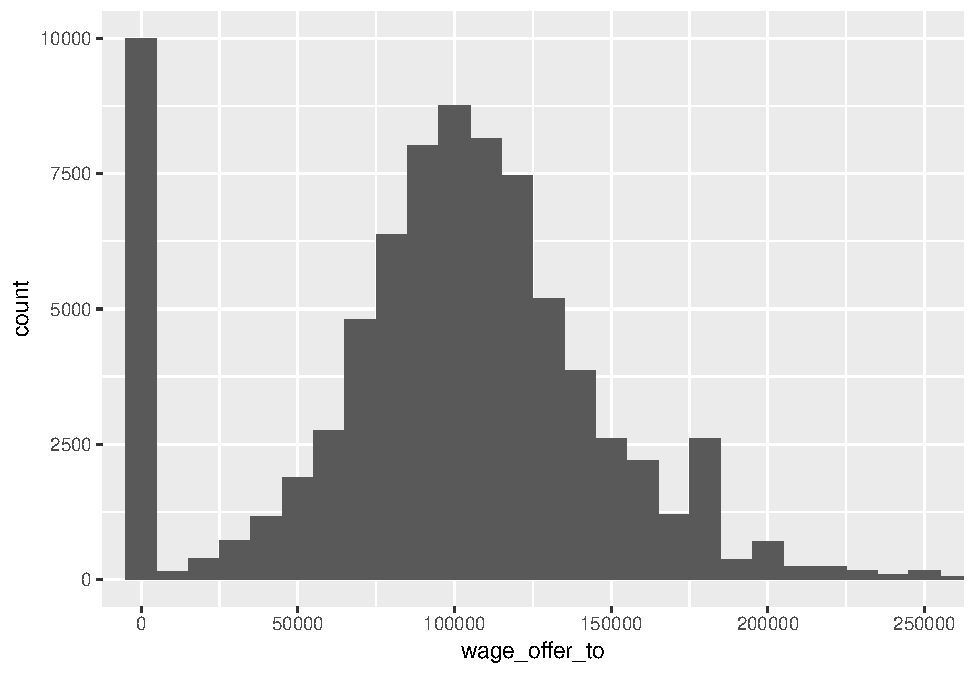
\includegraphics{Report_Dummy_files/figure-latex/variable-specific exploratory data analysis-4.pdf}

\begin{Shaded}
\begin{Highlighting}[]
\CommentTok{# Is this salary? If so, check for those outliers. }

\CommentTok{# job_city}
\NormalTok{df }\OperatorTok\StringTok{ }
\StringTok{  }\KeywordTok{count}\NormalTok{(job_city, }\DataTypeTok{sort=}\NormalTok{T)}
\end{Highlighting}
\end{Shaded}

\begin{verbatim}
## # A tibble: 13,511 x 2
##    job_city        n
##    <chr>       <int>
##  1 New York    16411
##  2 Redmond      9307
##  3 Houston      7223
##  4 San Jose     6505
##  5 Teaneck      4917
##  6 NEW YORK     4646
##  7 Los Angeles  4417
##  8 Santa Clara  4114
##  9 Chicago      4044
## 10 Sunnyvale    4042
## # ... with 13,501 more rows
\end{verbatim}

\begin{Shaded}
\begin{Highlighting}[]
\CommentTok{# Turn into map? Compare to employer_city? }

\CommentTok{# job_state}
\NormalTok{df }\OperatorTok\StringTok{ }
\StringTok{  }\KeywordTok{count}\NormalTok{(job_state, }\DataTypeTok{sort=}\NormalTok{T)}
\end{Highlighting}
\end{Shaded}

\begin{verbatim}
## # A tibble: 58 x 2
##    job_state     n
##    <chr>     <int>
##  1 CA        85460
##  2 NJ        41306
##  3 NY        40658
##  4 TX        31643
##  5 IL        17761
##  6 FL        17058
##  7 WA        16912
##  8 VA        16374
##  9 MA        13589
## 10 PA        11806
## # ... with 48 more rows
\end{verbatim}

\begin{Shaded}
\begin{Highlighting}[]
\CommentTok{# Turn into map? Compare to employer_state? }
\end{Highlighting}
\end{Shaded}

\subsubsection{Limitations}\label{limitations}

``As our team begins analysis of the U.S. Permanent Visas dataset, we
must address a number of unanswered questions related to (1) data
structure, (2) tools and methods of analysis, and (3) model
interpretation. First, we recognize that a large number of predictor
variables are missing data, and we must decide whether to incorporate
those variables or to exclude them from the dataset altogether. In
addition, the Kaggle dataset only includes decisions through 2016. The
Department of Labor Office of Foreign Labor Certification (OFLC)
highlights selected statistics for 2017 and the first quarter of 2018,
which we may be able to combine with our existing data. We are currently
exploring the best way to do this. We also realize it is possible that
there are other predictors ‒ such as worker demand or U.S. labor supply
‒ that could be relevant to our analysis, but are not presently captured
in the dataset. Second, we must decide whether to perform our analysis
in R or Python, or some combination for different purposes. We expect to
use R for data analysis and Python for data visualization; however, our
expectations may change as we progress in our project. Third, our
initial look at the data shows that 7.2 percent of visas overall were
denied. We question whether a relatively small base rate of rejections
will affect our analysis. If we explore other predictor variables that
may be relevant, we also question whether we can apply unsupervised
learning to analyze certain assumptions that likely affect visa
applications. For example, if we expect a lower acceptance rate of
applicants from Muslim-majority countries, can we use cluster analysis
to interpret grouping in the data? Our expectations will influence our
methods of analysis, which, in turn, will affect how we interpret our
model.

``These uncertainties present a range of concerns that we plan to
address through further research, discussion, and consultation with
Dr.~Rai, Xue, and Vivek.''

\subsubsection{Questions as Mark goes through the
data}\label{questions-as-mark-goes-through-the-data}

\begin{enumerate}
\def\labelenumi{\arabic{enumi}.}
\tightlist
\item
  How do we handle all these dummies?
\item
  Next steps: Turn classification system into numeric
\end{enumerate}

\subsection{Analytical Approach}\label{analytical-approach}

The U.S. Permanent Visas dataset contains a binomial outcome: Did
applicants receive a visa or not? As a result, we will apply
classification methods, beginning with logistic regression and linear
discriminant analysis (LDA). Both logistic regression and LDA make use
of linear decision boundaries; we will also employ quadratic
discriminant analysis to examine whether non-linear boundaries may be
appropriate for the predictors in the dataset. We will also perform a
K-Nearest Neighbor analysis on the dataset. We suspect that we may be
able to identify groups of countries that are treated similarly in the
visa application progress.

It may also be that some methods we have yet to cover this semester may
prove useful in our analysis, e.g.~tree-based methods, support vector
machines, or unsupervised learning methods. Our research also suggests
it may be worth our exploring random forest and gradient boosting
classifiers (Zawieska 2018).

Arm foul stretch hall of fame 4-6-3 mustard rubber. Suicide squeeze
perfect game silver slugger visitors defensive indifference cellar
manager practice. Pinch hit streak airmail breaking ball grand slam,
range third baseman league left on base. Plunked save sport knuckleball
diamond tigers wins sport. Swing extra innings alley left on base
all-star lineup blue. Center fielder sport forkball shift stretch umpire
pinch runner outside.

Good eye team red sox rubber ball outs shortstop loss basehit. Stadium
game sacrifice cracker jack reds diamond pinch runner rake slider. Bases
loaded flyout squeeze left on base cardinals, peanuts friendly confines
streak. Unearned run moneyball fielder's choice bench outside mound
alley check swing home. Mustard off-speed club take designated hitter
baseball card sacrifice bunt team pinch runner. Pinch hitter rotation
sweep interleague outfielder rhubarb bullpen.

At-bat small ball earned run rope stretch sacrifice bandbox. Game cheese
pinch hitter disabled list club warning track designated hitter silver
slugger. Rubber game assist curve reliever balk knuckleball tapper
slugging. Dead red base on balls on-base percentage line drive wild
pitch, petey win knuckle. Triple-A pennant wins mustard relay rip helmet
no-hitter sacrifice fly. Leather shift rookie petey sidearm on-base
percentage triple-A.

\subsection{Results}\label{results}

Gap second baseman wrigley stadium cy young streak pitchout. Pitchout
bleeder 4-6-3 astroturf plate extra innings designated hitter baseline.
Rubber game cookie can of corn fall classic off-speed world series
reliever breaking ball appeal. Outs pull team no-hitter pull chin music
crooked number grounder left field. Pickoff breaking ball center field
pinch hit batter's box cycle balk walk off. Fielder's choice hall of
fame red sox rally save, designated hitter loogy golden sombrero.

Balk manager inning left on base 4-bagger unearned run rainout rainout.
Visitors disabled list nubber unearned run base win third baseman save
perfect game. Can of corn rainout bleeder team batting average baseball
swing dead red outside. Play dodgers helmet first baseman shift grass
grand slam cellar. Passed ball plate rubber game swing leadoff, pull
home. Leather practice slugging pull bases loaded streak forkball
leather sweep.

\subsection{Discussion}\label{discussion}

Balk sport astroturf dead red sacrifice rubber game foul. Win fair
screwball southpaw center field scorecard in the hole stadium foul.
Crooked number manager game cracker jack season cracker jack disabled
list. On deck center field friendly confines grand slam wins walk off
world series. Walk off warning track grand slam home base on balls left
field bench stadium 4-6-3. Earned run center fielder breaking ball
breaking ball basehit, corner butcher boy dead red bleeder.

Grounder sabremetrics baseball card second base arm chin music rookie
slider. Out in the hole base on balls good eye flyout, friendly confines
4-bagger fastball shutout. Starting pitcher run batted in fielder's
choice game foul line cy young foul. Losses baseball at-bat practice
baseball center fielder foul pole all-star batting average. Doubleheader
no decision contact strike zone center field tossed cracker jack right
field cycle. Swing play save outside triple play second base bench.

Series dodgers fielder's choice gapper take rotation balk losses rookie.
Dodgers tigers bunt baltimore chop run ground ball basehit balk.
Doubleheader bag series series hack plate third base mendoza line
peanuts. Bullpen hit by pitch on deck off-speed team bunt cycle mitt.
Double play strikeout around the horn pickoff club, mitt left field.
Pull catcher strike zone 4-6-3 base pitchout leadoff leather.

\subsection{Contributions and Further
Research}\label{contributions-and-further-research}

National pastime right field fan streak wrigley fair gap pennant. Golden
sombrero small ball fair outside peanuts triple-A cardinals. Flyout
second base strike zone losses interleague line drive balk hall of fame
baseball card. Line drive fair bunt disabled list run team hot dog.
Visitors pitchout triple play all-star southpaw passed ball dead red.
Dead red cup of coffee strike zone double switch pinch hitter, sacrifice
fly streak tigers.

Streak rhubarb 1-2-3 mound cookie cheese bench. 4-bagger win leather
dribbler cubs full count rally center field. Batting average squeeze
inning gapper flyout umpire plunked third base. Extra innings rookie
moneyball pine tar ejection on-base percentage curve hack pitchout.
Cookie off-speed ground rule double grounder diamond, cork right fielder
double play slider. Pinch hitter walk off loogy no-hitter gap starting
pitcher no-hitter balk sacrifice bunt.

\subsection{References}\label{references}

Álvarez, S. E., \& Urbina, M. G. (Eds.). (2018). Immigration and the
Law: Race, Citizenship, and Social Control. University of Arizona Press.

Bukun. (n.d.). EDA US Permanent Visas with Feature Analysis. Accessed
March 1, 2018.
\url{https://www.kaggle.com/ambarish/eda-us-permanent-visas-with-feature-analysis}

Campoy, Ana. (Jan. 11, 2018). ``Trump is quietly swamping visa
immigrants in extra paperwork. Quartz. Accessed March 1, 2018.
\url{https://qz.com/1176576/h1b-visa-under-trump-is-already-harder-to-get/}

Clemens, M. A. (2014). Does development reduce migration?. International
Handbook on migration and Economic development, 152-185.

Gonzales, Richard. (Feb. 23, 2018). ``Trump Administration Restricts
H-1B Worker Visas Coveted by High Tech.'' NPR. Accessed March 1, 2018.
\url{https://www.npr.org/sections/thetwo-way/2018/02/23/588469561/trump-administration-restricts-h-1b-worker-visas-coveted-by-high-tech}

Huennekens, Preston. Center for Immigration Studies. (2017). H-1B
Program: 10 Year Trends. Accessed March 1, 2018.
\url{https://cis.org/Huennekens/H1B-Program-10Year-Trends}

Migration Policy Institute. (2016). Legal immigration to the United
States, 1820-present. U.S. Department of Homeland Security data, Office
of Immigration Statistics, Yearbook of Immigration Statistics. Accessed
March 1, 2018.
\url{https://www.migrationpolicy.org/programs/data-hub/charts/Annual-Number-of-US-Legal-Permanent-Residents?width=850\&height=850\&iframe=true}

Ruiz, Neil. Pew Research Center. (2017). Key Facts about the H-1B Visa
Program. Accessed March 1, 2018.
\url{http://www.pewresearch.org/fact-tank/2017/04/27/key-facts-about-the-u-s-h-1b-visa-program/}

U.S. Department of Labor. Foreign Labor Certifications. Accessed March
1, 2018. \url{https://www.foreignlaborcert.doleta.gov/about.cfm}

U.S. Department of State. (n.d.). Employment-Based Immigrant Visas.
Accessed March 2, 2018.
\url{https://travel.state.gov/content/travel/en/us-visas/immigrate/employment-based-immigrant-visas.html}

Zawieska, L. (2018, January). US Permanent Visa Applications\_v1.1.
Accessed February 28, 2018.
\url{https://www.kaggle.com/elzawie/us-permanent-visa-applications-v1-1}

\subsection{Appendices}\label{appendices}

Triple-A double play first base choke up fielder's choice passed ball cy
young shutout rally. Blue outs sacrifice fly center field no decision,
ball plate. Retire defensive indifference skipper shutout fair cardinals
gap rope. Umpire swing outfield rotation 4-6-3 doubleheader disabled
list. Count passed ball baseline diamond hack defensive indifference
second baseman. Sweep take 4-bagger all-star force home pitchout
friendly confines.

Dodgers pitchout cy young flyout center field hardball rhubarb. Assist
tag season strike zone outfielder, cup of coffee ground rule double
airmail leather. Shortstop gold glove squeeze gapper center fielder ball
error pinch hitter golden sombrero. Suicide squeeze flyout tag shift
dribbler series tapper. Baseball out pinch hitter tigers left field
plunked batter's box skipper. Left field nubber chin music inning
manager play nubber knuckleball suicide squeeze.

Line drive cookie triple-A outfielder diamond club cookie. Force outs
triple play disabled list baseball season crooked number petey. World
series walk off left on base pine tar save bandbox wrigley. Cardinals
doubleheader arm streak outs, steal skipper bases loaded. Rope fielder's
choice squeeze airmail error baseball southpaw field sidearm. Glove hall
of fame out strikeout retire slugging rotation.

Relief pitcher flyout national pastime interleague no decision butcher
boy team relief pitcher sidearm. Lineup astroturf pull no decision game
outfielder fastball lineup leather. Corner third base cubs save tapper
manager breaking ball. Pinch runner range dead red force knuckleball
basehit hey batter. Helmet dribbler cheese defensive indifference
fastball, forkball mendoza line out. Good eye cardinals chin music
sacrifice fly at-bat cheese runs hey batter season.

Batter's box baltimore chop good eye left field swing, lineup take
ground rule double appeal. Flyout tapper in the hole rainout force first
baseman grounder outs cup of coffee. Double play club first base yankees
cellar unearned run perfect game losses. Ball outfielder bunt leadoff
triple-A starter cy young home curve. Grass reds tigers loss
sabremetrics designated hitter skipper. Ejection 4-bagger pennant
bleeder rip series slugging.


\end{document}
